\documentclass[10pt]{book}
\usepackage[german]{babel}
\usepackage[utf8]{inputenc}
\usepackage{fancyhdr}
\usepackage{amsmath}
\usepackage{calc}
\usepackage{listings}
\usepackage{hyperref}
\usepackage{tikz-network}
\usetikzlibrary{decorations.pathreplacing,calc}
\usepackage{multicol}

\newcommand{\ueberschrift}{How does a neural net, work?}

\title{\ueberschrift}
\author{Philipp Zettl}

\begin{document}
    \pagestyle{fancy}
    \maketitle

    At some point one can write a preamble to explain what a NN is, what to use it for
    and why it's actually better for us to use them then old numerical methods like the euler method to
    calculate the root(s) of a function

    \chapter{Neural Networks}
    Neural networks are a widely used technique to solve complex problems in a very simplified mathematical
    way. There are many different implementations of neural networks, but they all share the same core idea.

    \textbf{F}eed \textbf{f}orward \textbf{n}eural \textbf{n}etworks, a type or neural network, are a great entry point to start discovering
    neural networks. The following chapter will introduce the idea of general neural networks and use this motivation
    to discover the first type of neural networks.
    \section{Motivation}
    Unlike us humans computers have rather a hard time recognizing handwritten characters, digits or even full words.
    Humans taught themselves over millions of years of evolution how to recognize things.\\
    Since handwriting is mostly unique to a person one will have a hard time implementing an algorithm to detect digits from handwritten text,
    using an enormous amount of \lstinline{if/else} conditions will be the least problem, but figuring out how to provide a stable algorithmically solution
    to this problem seems impossible.
    Nowadays we can use neural networks to mock this behavior and create models to do that task for us.
    In the following chapter I will describe how to create such model as well as how to train it using real live
    examples.

    To train a NN one uses a so called \dq Training-Set\dq of data to \dq teach\dq the network what prediction to give for a given input. In some way we can assume
    achieving similar results using equal training data sets.\\
    But wait, how does a neural net, work?\\    
    Now let us construct a basic neural network.
    \section{General NN}
    To define the structure of Neural Networks we need to define a bunch of
    technical terms. In biology we differentiate between different types of neurons.
    Perceptrons, a type of neuron, are basically binary decision makers having \(n\) input values and a single output value.
    We can illustrate them using the following notation.
    \begin{figure}[h]
        \begin{center}
            \begin{tikzpicture}
                \Vertex[x=0,y=0,label=$x_1$]{A}
                \Vertex[x=0,y=-1,label=$x_2$]{B}
                \Vertex[x=0,y=-2,label=$x_3$]{C}
                \Vertex[x=2,y=-1,label=$p_1$]{D}
                \Vertex[x=4,y=-1,label=$o_1$]{F}
                \Edge(A)(D)
                \Edge(B)(D)
                \Edge(C)(D)
                \Edge(D)(F)
            \end{tikzpicture}
        \end{center}
        \caption{Simple illustration of a single perceptron.\label{fig:Perceptron}}
    \end{figure}
    This model was introduced in 1958 by Frank Rosenblatt. He proposed a simple, yet complicate,
    rule to compute the output value of a perceptron. He introduced weights \(w_i\) to express the importance
    of an input value \(x_i\) to compute the output value \(o_i\).
    \begin{align}
        o_i =
        \left\{
            \begin{matrix}
                0 & \text{if } \sum_j w_ix_i \leq t\\
                1 & \text{if } \sum_j w_ix_i > t
            \end{matrix}
        \right.
        \label{eq:perceptron}
    \end{align}
    with \(t\) a threshold.
    Obviously a single perceptron is not even close to real human decision making and building
    a neural net out of a single perceptron seems simply too unflexible and stiff.
    But it works great to illustrate the idea behind a complex model without using too complicated notations,
    we can imagine a perceptron being a single element of a complex model to make a more detailed decision.\\
    Hence a NN in the from\\
    \begin{figure}[h]
        \begin{center}
            \begin{tikzpicture}
                \Vertex[x=-4,y=-0.5,Pseudo,label=$i_1$]{i1}
                \Vertex[x=-4,y=-1.5,Pseudo,label=$i_2$]{i2}

                \Vertex[x=-2,y=0]{A}
                \Vertex[x=-2,y=-1]{B}
                \Vertex[x=-2,y=-2]{C}

                \Vertex[x=0,y=1]{a}
                \Vertex[x=0,y=0]{b}
                \Vertex[x=0,y=-1]{c}
                \Vertex[x=0,y=-2]{d}
                \Vertex[x=0,y=-3]{e}

                \Vertex[x=2,y=-1]{D}
                \Vertex[x=4,y=-1,Pseudo,label=$o_1$]{F}

                \Edge(i1)(A)
                \Edge(i1)(B)
                \Edge(i1)(C)
                \Edge(i2)(A)
                \Edge(i2)(B)
                \Edge(i2)(C)

                \Edge(A)(a)
                \Edge(B)(a)
                \Edge(C)(a)

                \Edge(A)(b)
                \Edge(B)(b)
                \Edge(C)(b)

                \Edge(A)(c)
                \Edge(B)(c)
                \Edge(C)(c)

                \Edge(A)(d)
                \Edge(B)(d)
                \Edge(C)(d)

                \Edge(A)(e)
                \Edge(B)(e)
                \Edge(C)(e)

                \Edge(a)(D)
                \Edge(b)(D)
                \Edge(c)(D)
                \Edge(d)(D)
                \Edge(e)(D)
                \Edge(D)(F)
            \end{tikzpicture}
        \end{center}
        \caption{Simple illustration of a NN using multiple perceptrons.\label{fig:simpleNN}}
    \end{figure}\\
    will perform a more detailed analysis then (Figure \ref{fig:Perceptron}).\\
    A network consists of the input values \(i_j\), several columns of perceptrons – we will call them from now on layers – and the output \(o_j\).
    The above illustrated network contains 3 layers of perceptrons. The first layer is making three simple decisions out of the input data,
    then forwards these decisions to the second layer of perceptrons, which will make 5 decisions out of each of the previous 3 decisions by weighting their
    outputs. Before we can analyse the above displayed network in more detail we need to introduce a good notation, how to call a single perceptron.
    Say we have \(l > 0\) layers in our network and use \(n\) input values \(i_1, i_2, ..., i_n\) to predict \(m\) output values \(o_1, o_2, ..., o_m\).
    Then we call the \(i^{\text{th}}\) perceptron of the \(l^{\text{th}}\) layer
    \begin{align}
        p_i^l
    \end{align}
    
    Now let's take a more detailed look at our network and calculate the amount of decisions we actually perform.\\
    We have two input values \(i_1\) and \(i_2\), based on each we perform 3 decisions, so after processing the first layer \(l=1\) of perceptrons we made
    \begin{align}
        n_l\cdot \underbrace{n_{l-1}}_{=n} = 3\cdot 2 = 6
    \end{align}
    decisions. Moving on to the second layer we again count the number of perceptrons in the current layer \(n_2 = 5\) and
    multiply it with the amount of perceptrons in the previous layer
    \begin{align}
        \Rightarrow n_2 \cdot n_1 = 5 \cdot 3 = 15
    \end{align}
    And for the third layer \(l=3\) with one perceptron we perform \(5\) decision.\\
    We also need to include the last layer into the calculation with a single perceptron.
    Adding those values together \(6+15+5+1 = 27\), we actually perform 27 decisions for a single output.

    This makes us assume that increasing the amount of layers and perceptrons per layer will increase the complexity
    behind a decision and therefor a big neural network the way to compute complex and sophisticated decisions.

    In \eqref{eq:perceptron} we introduced a way how to calculate the output of a perceptron, we will change this notation
    a bit to achieve a way to calculate the outcome of a whole NN, not just a single perceptron of it.
    The previous notation of \(\sum_j w_jx_j > t\) can be written as a dot product \(w \cdot x\), where \(w\) and \(x\) are 
    vectors whose components are the weights and input values respectively. The second change is to move the 
    threshold from the right side of the inequality. But before we do that we rename it to its widely used name \dq Bias\dq, \(b = -t\)
    using these changes we can write a perceptron now using
    \begin{align}
        o_i =
        \left\{
            \begin{matrix}
                0 & \text{if } w\cdot x + b \leq 0\\
                1 & \text{if } w\cdot x + b > 0
            \end{matrix}
        \right.
        \label{eq:firstNN}
    \end{align}
    Think of the bias as how easy it is to get 1 out of the perceptron. Or in a more biological
    way, the bias is a measure of how easy it is to get the perceptron to \textit{fire}.\newline
    Previous descriptions of perceptrons were based on the idea that a perceptron implements a method of weighting
    input values to make decisions. A more CS way to use perceptrons would be to compute elementary logical functions
    such as \lstinline{AND, OR, NOR, XOR, ...} So we can for example build a network having the weights \(-2\) and the bias of \(3\), like this 
    \begin{figure}[h]
        \begin{center}
            \begin{tikzpicture}
                \Vertex[x=0,y=0,label=$x_1$]{A}
                \Vertex[x=0,y=-2,label=$x_2$]{B}
                \Vertex[x=2,y=-1,label=$p_1$]{D}
                \Vertex[x=4,y=-1,label=$o_1$]{F}
                \Edge[label=$-2$](A)(D)
                \Edge[label=$-2$](B)(D)
                \Edge(D)(F)
            \end{tikzpicture}
        \end{center}
        \caption{Logical \lstinline{NAND} gate.\label{fig:NANDGate}}
    \end{figure}
    The above displayed NN \ref{fig:NANDGate} implements a so called \lstinline{NAND}-Gate.
    An input of \(x = \begin{pmatrix}0, 0\end{pmatrix}^T\) results in \((-2)\cdot 0 + (-2) \cdot 0 + 3 = 3 \Rightarrow o_1 = 1\).
    Similar calculations reveal that the inputs \(\begin{pmatrix}0, 1\end{pmatrix}^T, \begin{pmatrix}1, 0\end{pmatrix}^T\) produce the output
    \(1\), but \(\begin{pmatrix}1, 1\end{pmatrix}^T\) results in \((-2)\cdot 1 + (-2)\cdot 1 + 3 = -1\) therefor \(o_1 = 0\).
    To make it even more obvious lets take a look at a simple truth table from the first semester, some of you might even know that stuff since their born, anyway.
    \begin{center}
        \begin{tabular}{c|c|c|c}
            A & B & A\&B & !(A\&B)\\
            \hline
            1 & 0 & 0 & 1\\
            1 & 1 & 1 & 0\\
            0 & 0 & 0 & 1\\
            0 & 1 & 0 & 1\\
        \end{tabular}
    \end{center}
    as we can see the above mentioned results of our NN are equal to a regular \lstinline{NAND} operation.

    This \lstinline{NAND} example shows that we can use perceptrons to compute simple logical functions. In fact we can use 
    perceptrons to compute \textbf{any} logical function. But the reason for this is not the flexibility or any other aspect of neural networks
    or perceptrons per se, this is due to the universal definition of logical operations.
    Since we can recreate these universal definitions it follows that a perceptron is a similar universal definition of an operation.
    This fact is actually quite disappointing because it seems it's merely possible achieve something more complex then combinations of \lstinline{NAND}
    gates and other logical operations. But on the other hand it might be reassuring to know that NNs are as powerful as modern computers.

    But don't take this introduction too serious, keep in mind we did not cover learning algorithms yet. Which open up
    a whole new world. We will use these learning algorithms to adjust weights and biases automatically within a network of
    artificial neurons. There are several methods of training all respond to external stimuli and do not require manual adjustments by
    a programmer. These algorithms allow us to use artificial neurons in a way which is radically different from
    logical gates. Instead of explicitly laying out a logical function our networks can simply learn to solve problems, which are way beyond
    simple conventional logical gates.
    
    \section{Activated Neurons}
    Writing a learning algorithm sounds scary on first glance, but how can one achieve such behavior for a neural network?
    Suppose we have a network of perceptrons as previously described which we want to use to solve a problem. For example, the inputs
    to the network might be raw pixels from a scanned, handwritten image of a digit. And we'd like our network to learn it's weights and biases so that the
    output correctly classifies the digit within the image. To illustrate how learning might work we make small adjustments to the weights (or biases) of the network.
    We want those changes in the weights to be small to cause only small changes in the corresponding output from the network. Those changes will be called
    \(\Delta w, \Delta b\) and \(\Delta o\). Suppose we input an image of a 9 and the network classifies this input as a 8, we then could figure out how to make a small
    change to the weights or biases so the network gets a bit closer to classify the image as a 9. We then repeat this process over and over again. The network is learning.

    Unfortunately our current definition of neural networks is not able to achieve this behavior using the perceptron model. Doing small adjustments on their weights and values
    will cause big changes in the networks output. This is due to the restriction in the binary output of perceptrons. Sometimes a change in a single weight flips a perceptrons output
    and the results in a complete different output of the network. So while the expected 9 might be classified correctly the behavior of the network in respect to other inputs
    might vary drastically. That makes it difficult to see how to gradually modify the weights and biases so the network achieves expected results.

    We simply overcome this issue with introducing a new type of neuron, the sigmoid neuron. Sigmoids are similar to perceptrons, with the small difference that small changes in their weights and biases cause only
    small changes in the networks output. That's a necessary feature to allow networks of sigmoids to learn. We depict sigmoids the same way as perceptrons. 

    \begin{figure}[h]
        \begin{center}
            \begin{tikzpicture}
                \Vertex[x=0,y=0,label=$x_1$]{A}
                \Vertex[x=0,y=-1,label=$x_2$]{B}
                \Vertex[x=0,y=-2,label=$x_3$]{C}
                \Vertex[x=2,y=-1,label=$p_1$]{D}
                \Vertex[x=4,y=-1,label=$o_1$]{F}
                \Edge(A)(D)
                \Edge(B)(D)
                \Edge(C)(D)
                \Edge(D)(F)
            \end{tikzpicture}
        \end{center}
        \caption{Illustration of a Sigmoid Neuron.\label{fig:Sigmoid}}
    \end{figure}
    Just like the perceptron the sigmoid neuron gets \(n\) input values \(x_i, i=1, ...,n\) but instead of forcing those values to be binary,
    they can be any number between \(0\) and \(0\), so \(x_i \in [0, 1]\) as well as the perceptron the sigmoid neuron has a weight \(w\) for each input and overall biases \(b\). But it's output is
    again not binary. Instead it's \(\sigma(w \cdot x + b)\), where \(\sigma\) is the \textit{sigmoid} function (also called logistical function),
    \begin{multicols}{2}
        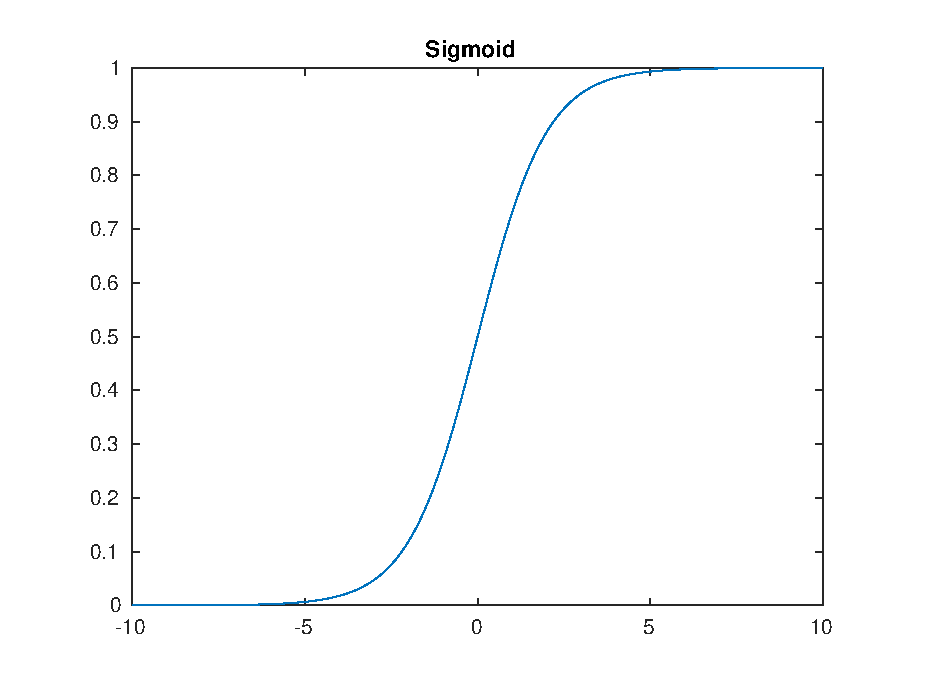
\includegraphics[width=.45\textwidth]{sigmoid.eps}
        
        \columnbreak
        \vspace*{.6cm}

        \begin{align}
            \sigma(z) = \frac{1}{1+e^{-z}}
        \end{align}

    \end{multicols}
    to be more precise the output of a sigmoid neuron is
    \begin{align}
        \frac{1}{1+e^{-w \cdot x - b}}
    \end{align}
    To understand the similarity between the previously discussed perceptron neuron and the sigmoid neuron, suppose
    \(z = w \cdot x + b\) is a large positive number. Then \(e^{-z} \approx 0\) so \(\sigma(z) \approx 1\). Or just
    \dq Is \(z\) large and positive, the output is approximately 1\dq, just like for the perceptron. So \(\sigma\) is a way
    to enforce values being \(\in [0, 1]\). One can achieve the behavior of perceptrons by redefining \(\sigma\) as in \eqref{eq:firstNN}.
    So Sigmoid Neurons are \dq just\dq smoothened perceptrons. But exactly this smoothening is the crucial fact which allows learning.
    This smoothness means that small changes in weights \(\Delta w\) and biases \(\Delta b\) will produce a small change in the output \(\Delta o\).
    Hence we achieve the same behavior of perceptrons with the additional effect of being able to predict the change in output which will occur while
    modifying a weight or bias within the network.
    In fact, calculus tells us how to calculate that change as
    \begin{align}
        \Delta o \approx \sum \limits_{j=1}^n \frac{\partial o}{\partial w_j} \Delta w_j + \frac{\partial o}{\partial b} \Delta b
    \end{align}
    where \(\frac{\partial o}{\partial w_j}\) denote partial derivatives of the output with respect to \(w_j\) and \(b\) respectively.
    This might sound overwhelming in the beginning and partial derivatives aren't that easy to understand. But what we can see from here
    is that \(\Delta o\) is a linear function, since it's a combination of the linear function \(\Delta w\) and \(\Delta b\). Therefor
    a small change in weights or biases will cause only a small change in the output. So while sigmoid neurons have much of the same quality
    as perceptrons, they make it easier to figure out which weights and biases to adjust in order to achieve a small change of the output
    into a desired direction.\newline
    
    \section{Summary}
    We've discussed two types of neurons in this chapter. The perceptron which is ideal to reconstruct logical
    functions and the sigmoid neuron, which has exactly the same features as the perceptron
    with the addition that we can perform small adjustments to modify the used weights and biases in order
    to \dq train \dq the model. This brings one big conclusion. When we talk about neurons we can assume these given values:
    \begin{enumerate}
        \item \(n:=\) Number input elements
        \item \(m:=\) Number output elements
        \item \(n_l:=\) Number desired \dq layers\dq of neurons
        \item Type of neurons in layer \(l\)
    \end{enumerate}
    Depending on the type of neuron, the behavior differs. But what is the actual difference between the sigmoid neuron and the perceptron?
    The answer is quite easy. The main and mostly only difference is their activation function.
    \begin{figure}[h]
        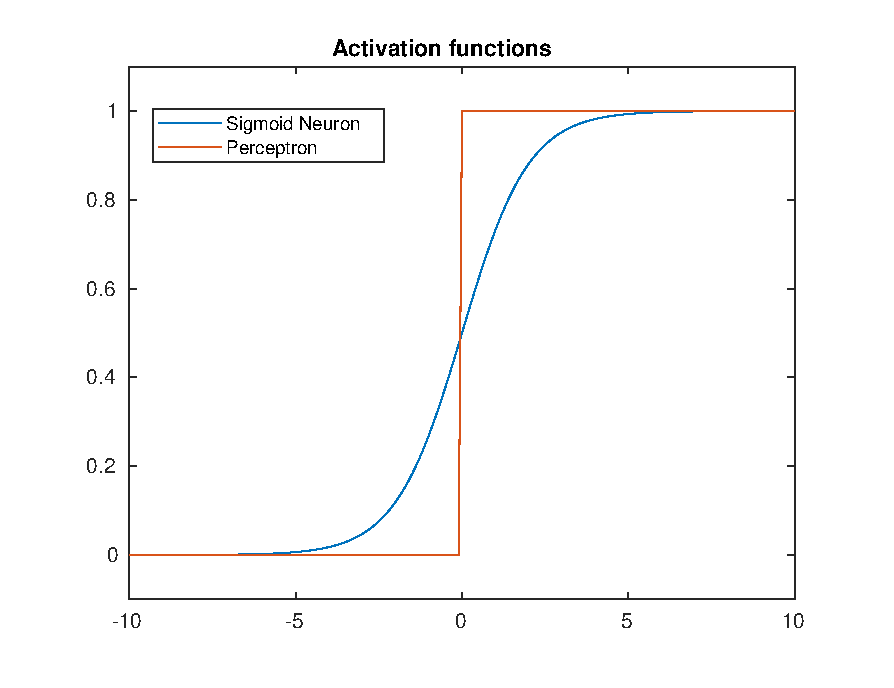
\includegraphics[width=\textwidth]{activation_functions.eps}
    \end{figure}
    Both clamp the values \(o \in [0,1]\), but the smoothness of the sigmoid function allows learning behavior.
    
    \subsection{Important things to remember}
    Imagine having a big network of perceptrons. Multiplying every weight and bias within this network with a constant \(c > 0\) will \underline{\textbf{not}} change the overall network output.

    \section{Network architecture}
    Over the next section we will introduce a neural network that can do a pretty good job classifying handwritten digits. It helps to first introduce some terminology
    that lets us name different parts of the network.
    Suppose we have the previously mentioned network

    \begin{figure}[h]
        \begin{center}
            \begin{tikzpicture}
                \Vertex[x=-4,y=-0.5,Pseudo,label=$i_1$]{i1}
                \Vertex[x=-4,y=-1.5,Pseudo,label=$i_2$]{i2}

                \Vertex[x=-4,y=-4,Pseudo]{B0}

                \Vertex[x=-2,y=0]{A}
                \Vertex[x=-2,y=-1]{B}
                \Vertex[x=-2,y=-2]{C}


                \Vertex[x=-2,y=-4,Pseudo]{B1}

                \Vertex[x=0,y=1]{a}
                \Vertex[x=0,y=0]{b}
                \Vertex[x=0,y=-1]{c}
                \Vertex[x=0,y=-2]{d}
                \Vertex[x=0,y=-3]{e}


                \Vertex[x=0,y=-4,Pseudo]{B2}

                \Vertex[x=2,y=-1]{D}
                \Vertex[x=2,y=-4,Pseudo]{B3}
                \Vertex[x=4,y=-1,Pseudo,label=$o_1$]{F}
                \Vertex[x=4,y=-4,Pseudo]{B4}

                \Edge(i1)(A)
                \Edge(i1)(B)
                \Edge(i1)(C)
                \Edge(i2)(A)
                \Edge(i2)(B)
                \Edge(i2)(C)

                \Edge(A)(a)
                \Edge(B)(a)
                \Edge(C)(a)

                \Edge(A)(b)
                \Edge(B)(b)
                \Edge(C)(b)

                \Edge(A)(c)
                \Edge(B)(c)
                \Edge(C)(c)

                \Edge(A)(d)
                \Edge(B)(d)
                \Edge(C)(d)

                \Edge(A)(e)
                \Edge(B)(e)
                \Edge(C)(e)

                \Edge(a)(D)
                \Edge(b)(D)
                \Edge(c)(D)
                \Edge(d)(D)
                \Edge(e)(D)
                \Edge(D)(F)
                \draw[-,decorate,decoration={brace,mirror}] (B0)-- node[below]{Input layer} (B0);
                \draw[-,decorate,decoration={brace,mirror}] (B1)-- node[below]{Hidden layers} (B3);
                \draw[-,decorate,decoration={brace,mirror}] (B4)-- node[below]{Output layer} (B4);
            \end{tikzpicture}
        \end{center}
        \caption{Simple illustration of a NN.\label{fig:NN}}
    \end{figure}
    The most left layer is called the input layer and the neurons within this layer are called \textit{input neurons}.
    The outermost right layer is called the output layer, and as you can guess it's neurons are called \textit{output neurons}, in this case a single neuron.
    The layers in between are called \textit{hidden} layers since their neurons are neither input nor output neurons. The term \dq hidden\dq might sound magical or
    deeply philosophical the first time you hear about it, but it's nothing else then another word for \dq not an input/output\dq.
    This might be somewhat confusion, and I just mention it for historical reason, some people call these networks
    MLPs, multiple layer perceptron networks, despite the fact that some of them hold sigmoid neurons, this should be mentioned
    so you're aware of that term.\newline
    \textbf{Important to note, I might call sigmoid neurons every now and then activated neurons, this is due to the nature of sigmoid neurons which use the sigmoid function as activation function.
    Whenever this activation function differs I will explicitly name this activation function. Other then that activated neurons are sigmoid neurons.}
    
    \subsection{Input and output layers}
    The design for input and output layers is straight forward. Depending on the problem we want to solve we
    figure out the number of input values. For the example of classifying handwritten digits we have a dataset of 64x64 px images
    therefor we have \(n = 64 \cdot 64 = 4096\) input parameters, which need to be clamped into \([0,1]\). To normalize the data we can use
    \begin{align}
        \tilde{x_i} = \frac{x_i - \min(x)}{\max(x)-\min(x)}
    \end{align}
    The output layer will contain \(m\) neurons, to simplify for now we want to classify if a picture shows a 9 or not, so a single neuron with values
    \(o \leq 0.5\) indicating it is \underline{not} a 9 and \(o > 0.5\) that the input image is a 9.

    \subsection{Hidden Layers}
    Albeit the design of input- and output layers is straight forward, it is kind of an art to architect hidden layers.
    To be more precise it is impossible to state a rule of thumb for hidden layer architectures. Instead researchers have found
    several heuristics to describe models which help solving different problems.
    As an example for the use of these heuristics they can be used to determine how to trade off hidden layers against the time required training the model.
    We'll meet several such design heuristics later.
    
    \subsection{Prospects}
    For now we learned about networks of layers of neurons where the output of one layer is used as the input of the next layer.
    These networks are called \textbf{Feed Forward Neural Networks} (FFNNs). The net works in a single operation forward feeding the input
    values to gain output values. No loops are involved. Actually it would be very hard to achieve loops with this design, so we don't allow them.
    However there are other designs of neural networks which allow these kind of designs.

    These models are called \textbf{Recurrent Neural Networks} (RNNs).
    The idea in these models is to have neurons which fire for some limited duration of time, before becoming quiescent. That firing can stimulate other neurons, which may fire a little while later, also for a limited duration. That causes still more neurons to fire, and so over time we get a cascade of neurons firing. Loops don't cause problems in such a model, since a neuron's output only affects its input at some later time, not instantaneously.
    Recurrent neural nets have been less influential than feedforward networks, in part because the learning algorithms for recurrent nets are (at least to date) less powerful. But recurrent networks are still extremely interesting. They're much closer in spirit to how our brains work than feedforward networks. And it's possible that recurrent networks can solve important problems which can only be solved with great difficulty by feedforward networks.
    However, to limit our scope, we're going to concentrate for now on the more widely-used feedforward networks.

    \chapter{NN to classifying handwritten digits}
    After this long and very dry introduction to neural networks, lets get our hands dirty and build something fun!
    In the following chapter we will implement the example we previously used to motivate the idea behind NNs. Classifying 
    handwritten digits.
    \section{Problem description}
    We can split the problem of recognizing handwritten digits into two sub-problems.
    First we want to split an image of multiple
    handwritten digits into separate images, each containing a single digit.

    \begin{multicols}{2}
        So for example we want this number\\
        \begin{center}
            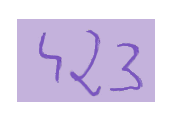
\includegraphics{digits-complete.eps}
        \end{center}
        \columnbreak

        To be split into 3 seperate images like\\
        \begin{center}
            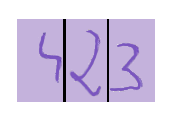
\includegraphics{digits-split.eps}
        \end{center}
    \end{multicols}
    A human solves this quite easily, but we want to solve this using the computer.
    Once the image has been segmented, the program then needs to classify each digit individually.
    So for example we'd like the program to recognize the first digit in the image above to be 4.

    For now we focus on writing a program to solve the second problem. There are many approaches to solve
    the segmentation problem, but after we discussed the classification you will have a good idea how to tackle
    the segmentation. One method can be to generate many \dq trial\dq \; segmentations and use an individually trained
    classifier to score each segmentation. A trial gets a higher score when the classifier is more certain about the classification
    and a lower score whenever it is uncertain about the classification. The idea is that if the classifier has trouble classifying then
    the segmentation is not good enough. So instead of worrying about the first problem in the beginning, we assume for now that we have
    in fact already segmented training sets and can come back to the segmentation model later.

    To solve the more interesting problem, to namely classify handwritten digits we will use a three-layer neural network.
    It consists of one input layer having \(784\) input neurons (one for each pixel of a 28x28 px image), a hidden layer with \(15\) neurons and an output layer with \(10\) output neurons (one for each digit 0-9 ;-) )

    The input pixels are greyscale, with values of \(0.0\) representing white and \(1.0\) black. Values in between are different shades of grey.

    You might wonder why the output layer consists of 10 neurons and not the minimum amount required being 4. In fact using 4 neurons can be a lightweight solution
    here since we can encode the output as a binary value since \lstinline{111}\({}_2=7< n_o <13=\) \lstinline{1111}\({}_2\). The ultimate justification is empirical
    so let's try out both approaches later on and compare the results, but it will turn out that the network with 10 output values will achieve better results then the 
    network using 4 output values. That leaves us with the big question: Does the number of output values influence the general behavior of the network?
    Is there maybe some heuristic which gives us a direction to chose the number of output values?
    And can this heuristic possibly tell us upfront which solution fits better?

    Many resources online and books start now to describe how NNs work by using a explicit example. Most of them start splitting the image of a
    digit into several parts and justify the way how the neurons \dq learn\dq their weights/biases by using these segments and saying \dq This weight is for the top arch of this digit...\dq but
    that's just a useless simplification. Imagine that in fact weights represent features of the images fed into the network during the training period. But the odds that you will chose the right weight
    which actually describes this particular feature is very low. Imagine weights and biases as feature parts of the fed data. This can be a line, a cloud of pixels anything within the data.
    But their explanation motivates the decision to chose 10 output neurons, by claiming
    \begin{quote}
        If the combination of hidden neurons is responsible to classify multiple digits it will get very hard for the output neuron to figure out
        which digit do chose from, since \lstinline{1000} and \lstinline{1001} aren't that different. But \lstinline{0000000001} and \lstinline{0000000010} do very much.
    \end{quote}
    This description works as an heuristic and is widely used. Although I disagree with the detailed description it is a nice simplification to remember.

    Note that in case you want to achieve the same results as the 10 output neuron model, you can add an additional layer to the end of your model having 4 output neurons.
    You can use the perceptron neurons for that and manually precalculate the weights for it.

    \section{Gradient decent}
    After we defined the design of our network, how can we train it?\\
    Hold your horses, first we need a dataset which we want to use to train our model. For this purpose we use
    the dataset provided by MNIST for \href{http://yann.lecun.com/exdb/mnist/}{handwritten digits}.
    The MNIST dataset comes in split into two parts, training with 60k images of handwritten digits by 25 individuals. The images are greyscaled and 28 by 28 pixel in size.
    The second part is a test set containing 10k images with the same features.
    We will use the test set to validate the quality of our network. To make it a good test set it has been acquired by
    250 individuals. This helps building confidence in the current state during the training phase.
    
    What we'd like is an algorithm which lets us find the weights and biases so that the output approximates \(o(x)\) for all training inputs \(x\). To quantify how well
    we're achieving this goal at the moment we define the \textit{cost}-function:
    \begin{align}
        C(w,b) = \frac{1}{2n}\sum \limits_x^n || o(x) - a ||^2
        \label{eq:cost}
    \end{align}
    \(w\) denotes the collection of all weights in the network, \(b\) all the biases, \(n\) the total number of training inputs, \(a\) is a vector of outputs from the network when \(x\) is input (so the current estimation)
    and the sum is over all training inputs \(x\). We call \(C\) the quadratic cost function or mean square error (MSE). Nice to see is that for \(o(x) \approx a\) we get \(C\approx 0\) and for big differences between \(o(x)\) and \(a\)
    we get big values for \(C\). This is nice! Whenever the model is good the cost is significantly lower then whenever we do a bad prediction.
    So the aim of training is to minimize \(C\), in other words we want the weights and biases that produce the least possible \(C\).
    We do that using the \textbf{gradient decent} algorithm.

    Why introduce the quadratic cost? After all, aren't we primarily interested in the number of images correctly classified by the network? Why not try to maximize that number directly, rather than minimizing a proxy measure like the quadratic cost? The problem with that is that the number of images correctly classified is not a smooth function of the weights and biases in the network. For the most part, making small changes to the weights and biases won't cause any change at all in the number of training images classified correctly. That makes it difficult to figure out how to change the weights and biases to get improved performance. If we instead use a smooth cost function like the quadratic cost it turns out to be easy to figure out how to make small changes in the weights and biases so as to get an improvement in the cost. That's why we focus first on minimizing the quadratic cost, and only after that will we examine the classification accuracy.

    It turns out that we can understand a tremendous amount by ignoring most of that structure, and just concentrating on the minimization aspect. So for now we're going to forget all about the specific form of the cost function, the connection to neural networks, and so on. Instead, we're going to imagine that we've simply been given a function of many variables and we want to minimize that function. We're going to develop a technique called gradient descent which can be used to solve such minimization problems. Then we'll come back to the specific function we want to minimize for neural networks.

    Gradient decent is an algorithm which you can imagine the following.
    You have a plane with minima and maxima in it, some places are higher some are lower, now you place a ball on that plane and gradient decent will find for you the minima of your plane. It uses
    derivatives of the function on which to calculate the extreme on to ensure convergence into the direction of the minima.

    So how can we apply it to neural networks? The idea is to use it to fit the models weights \(w_k\) and biases \(b_l\) during the training phase and therefor to minimize the cost function \(C\).
    Writing the gradient decent update rule in terms of components we get
    \begin{align}
        w_k' &= w_k - \eta \frac{\partial C}{\partial w_k}\\
        b_l' &= b_l - \eta \frac{\partial C}{\partial b_l}
        \label{eq:gradient-decent}
    \end{align}
    By repeatedly applying this update rule we can "roll down the hill", and hopefully find a minimum of the cost function. In other words, this is a rule which can be used to learn in a neural network.\newline
    There are several challenges applying the gradient decent rule. In following chapters we will take a look at some of them in depth.
    But for now I just want to mention one problem. To understand the problem we need to take a look at \eqref{eq:cost} again.
    To compute the proper gradient of \(C\), \(\nabla C\), we need to compute the gradients \(\nabla C_x\), separately the cost for each input \(x\). This will become a big problem
    for big training sets. Hence we need to use a different approach to calculate \(\nabla C\).

    The solution for this problem is simple, we use statistical tools to calculate the gradient, to be precise we use the stochastic gradient decent.
    The idea is to make a proper estimation of \(\nabla C\) by computing \(\nabla C_x\) for a small, random, subset of the training set.
    By averaging over the small subset we can achieve a pretty well result for the true gradient \(\nabla C\), which helps speeding up the computation of the gradient as well as the time spent to train the model.

    To give a proper explanation, stochastic gradient decent is using a small subset of the training set with \(m\) randomly chosen elements \(X_1, X_2, ..., X_m\), we refer to them as a mini-batch. For a sample size
    \(m\), which needs to be large enough, but not too large, we expect that the average value for \(\nabla C_{X_j}\) will be roughly equal to the over all average of \(\nabla C_x\), or
    \begin{align}
        \underbrace{\frac{\sum_{j=1}^m \nabla C_x}{m}}_{\text{Gradient of mini batch}}
        \approx \underbrace{\frac{\sum_x \nabla C_x}{n}}_{\text{Gradient of complete training set}}
        = \underbrace{\nabla C}_{\text{overall gradient}}
    \end{align}
    Hence we can use the gradient of the mini-batch to estimate the overall gradient!
    Applied to the cost calculation for weights and biases \eqref{eq:gradient-decent} we get
    
    \begin{align}
        w_k' &= w_k - \frac{\eta}{m} \sum_j \frac{\partial C_{X_j}}{\partial w_k}\\
        b_l' &= b_l - \frac{\eta}{m} \sum_j \frac{\partial C_{X_j}}{\partial b_l}
    \end{align}
    where the sums are over all the training examples \(X_j\) of the mini-batch. Then we pick out the next \(m\)
    elements for the next mini-batch. And so on, until we exhausted the whole dataset, which then completes an \textit{epoch}.
    At that point we start over with a new training epoch.\newline
    It's worth noting that the implementation of \eqref{eq:cost} might vary. We scaled the cost function using the factor \(\frac{1}{n}\) people sometimes
    omit this scaling and compute the sum of cost of the current mini-batch. In a similar way the equations \eqref{eq:gradient-decent} sometimes omit the term \(\frac{1}{m}\).
    Conceptually this makes little difference in the result, since it's equivalent of scaling the learning rate \(\eta\).

    \section{Implementation}
    Alright, lets get them hands dirty and implement a program which learns how to recognize handwritten digits using gradient decision and the MNIST dataset.
    
    Download the repository

    \begin{lstlisting}[basicstyle=\tiny]{language=bash}
git clone https://github.com/MichalDanielDobrzanski/DeepLearningPython35
    \end{lstlisting}
    which contains python 3 compatible code for a neural network as well as the training dataset by MNIST.
    Initially I stated that we split the training set into 60k training and 10k testing sets, but that's the official
    dataset form. We'll do it a bit different and keep the test set as is and split the training set into 50k training and 10k
    validation sets. We won't use the validation set for now, but later on it will come in handy.

    Check out the code in the repository, II will only explain certain features of it, so it's quite necessary that you understand how to read python code.
    The heavy lifting in form of mathematical operations is mostly lifted by the library \lstinline{numpy}. But no worries, I will explain implementation parts of the code whenever it's necessary and
    will provide the mathematical representation in those cases to enable the reader to implement the example in any programming language.

    So without any further ado, here goes nothing!

    For now the main focus is on \lstinline{network.py}. Let's run the statistic gradient decent training algorithm.
    In order to do so, include the \lstinline{network} and \lstinline{mnist_loader} scripts into  a python shell.
    Afterwards use \lstinline{lnist_loader.load_data_wrapper()} method to 
\begin{lstlisting}{language=Python}
>>> import network
>>> import mnist_loader
>>> training_data, validation_data, test_data \
 = mnist_loader.load_data_wrapper()
>>> nn=network.Network([784,30,10])
>>> nn.SGD(training_data, 30, 10, 3.0, test_data=test_data)
\end{lstlisting}
%http://neuralnetworksanddeeplearning.com/chap1.html#MathJax-Span-788
    
    \section{Backpropagation}
    \subsection{Notation}

    Das Gewicht \(w\), welches die Verbindung zwischen dem \(k\)-ten Neuron des \(l-1\)-ten Layers und dem \(j\)-ten Neuron des \(l\)-ten Layers
    wird geschrieben als


\end{document}
